\documentclass[a4paper,11pt,titlepage]{jarticle}
\usepackage[dvipdfmx]{graphicx}
\usepackage{listings}
\usepackage{amsmath}
\usepackage{fancybox,ascmac}

\title{知能情報実験I : 第七回レポート}
\author{175751C 宮城孝明}
\date{\today}

\begin{document}
\maketitle
\tableofcontents
\clearpage
\section{実験目的}
 現代社会に欠かすことのできないコンピュータは,大規模なディジタル回路として構成されている。本実験では,ディジタル回路の構成要素である基本ゲート回路と論理演算の基礎を習得することを目的としている。また本実験では,NAND(NOT,AND,OR,NOR,XOR)を構成することによって,汎用ロジックICおよびブレッドボード,直流電源などの基本的な使用法についても学ぶ。\par

\section{実験概要}
 今回の実験は,ディジタル回路の基本構造を理解するために,実際の回路作成を行った。まず始めに,NANDだけを用いてNOT,AND,OR,NOR,XOR回路を紙の上で回路図として表現した。回路作成する際に,全体の見取り図として,これを役立てた。そして,回路作成にあたり教授たちが前で基本的な説明や取り扱い際の諸注意をした。あらかじめ用意してもらった汎用ロジックとブレッドボード,直流電源を用いて,先ほどの回路を作成する作業に移る。そして,出力結果を確かめるために,LEDの灯が付くか付かないで確認をした。そのため,私たち学生でも自作の回路が適切かどうか判断できる。さらに,教授や院生,外部の人たちが学生の質問に回って答えたり,実際の動作を一緒に確認した。\par


\section{実験結果}
実験(1)\par
ここは,NANDゲートを用いてNOT,AND,OR,NOR,XORゲートを再現する。\par
\begin{figure}[htbp]
  \centering
  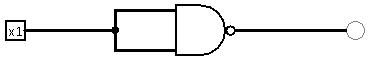
\includegraphics[width=100mm]{sample4.png}
  \label{sample1}\\
  \caption{NANDゲートで示したNOT回路}
\end{figure}
\par
\begin{figure}[htbp]
  \centering
  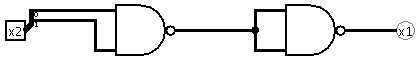
\includegraphics[width=100mm]{sample5.png}
  \label{sample2}\\
  \caption{NANDゲートで示したAND回路}
\end{figure}
\par
\begin{figure}[htbp]
  \centering
  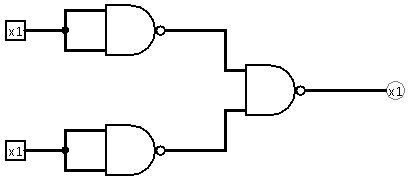
\includegraphics[width=100mm]{sample6.png}
  \label{sample3}\\
  \caption{NANDゲートで示したOR回路}
\end{figure}
\par
\begin{figure}[htbp]
  \centering
  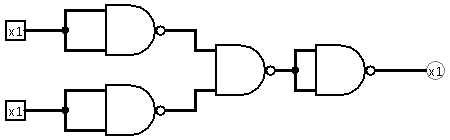
\includegraphics[width=100mm]{sample7.png}
  \label{sample4}\\
  \caption{NANDゲートで示したNOR回路}
\end{figure}
\par
\begin{figure}[htbp]
  \centering
  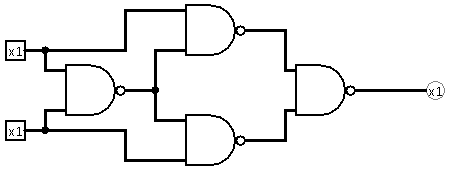
\includegraphics[width=100mm]{sample8.png}
  \label{sample5}\\
  \caption{NANDゲートで示したXOR回路}
\end{figure}
\par
\begin{figure}[htbp]
  \centering
  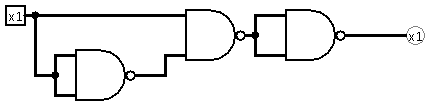
\includegraphics[width=100mm]{sample14.png}
  \label{sample6}\\
  \caption{NANDゲートで示した常に0を出力する回路}
\end{figure}
\par
\begin{figure}[htbp]
  \centering
  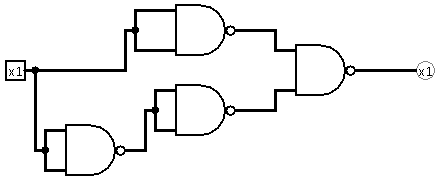
\includegraphics[width=100mm]{sample15.png}
  \label{sample7}\\
  \caption{NANDゲートで示した常に1を出力する回路}
\end{figure}
\par

図1は,NOT回路となっている。NOT回路は,出力結果が入力の値を否定になる。そして,NAND回路は入力(0,0)の場合は1を出力,入力(1,1)の場合は0を出力する。そのため,一度入力を二つに分ける。こうして,入力に対してその否定を出力するNOT回路が完成する。\par
この回路図に初めに0を入力する。入力を2分にして,NANDに入れる。そのため,NAND回路には入力(0,0)が入力されたことになる。よって、出力結果は,0となる。同様に,1を入力したら出力は0になる。\par
図2は,AND回路となっている。AND回路は,入力(1,1)の時だけに出力1を返す。つまり,NOND回路をNOT回路で否定した回路になることが予測できる。よって,初めにNAND回路に値を入力し,その出力を1番目に作成したNOT回路で否定することでAND回路は完成する。\par
この回路に(0,0),(1,0),(0,1)を入力したら最初のNAND回路で1の値になる。それを次のNOT回路で否定することで出力結果は,0となる。(1,1)という入力では最初のNAND回路で0の値になり、NOT回路で1という出力になる。よって、AND回路の完成になる。\par
図3は,OR回路になる。OR回路は入力値(0,0)以外は1を返すという回路である。つまり,初めの入力値を否定しそれをNAND回路で出力することでOR回路は完成する。\par
この回路に,(1,1),(1,0),(0,1)を入力する。始めの否定回路により,全ての値は反対になる。その際,値に(1,1)はない。そのため,この3入力は出力結果は必ず1が返ってくる。しかし、入力値を(0,0)した場合,否定回路で(1,1)となる。これにより,出力結果は0が返る。\par
図4は,NOR回路である。この回路は,OR回路の否定であるため,先ほど作成したOR回路に否定のNOT回路を付け加えれば完成する。\par
OR回路の否定ため,2つ目のNAND回路で値が1になったり0になったりたのを否定する。この回路に,(1,1),(1,0),(0,1)
を入力したら0を返し,(0,0)の入力値に対しては1に返す。\par
図5は,XOR回路である。入力値をNAND回路を取り入れ,その値を初めの値たちでNANDを取り,さらにその値をNANDを取ることによって,完成する。\par
この値に(1,0),(0,1)を入力すれば,始めのNAND回路で1を出力する。そして,次のNAND回路で片方は0をもう片方は1を出力する。これにより,最後のNAND回路で値は1を出力する。しかし,(1,1),(0,0)を入力したら,始めのNAND回路で入力値の値は反対になる。それにより,2つ目のNAND回路両方とも1を出力する。そして,最後のNAND回路で0が出力される。\par
図6は,常に出力値0になる回路図である。そのためには,入力値とその値の補集合の論理積を取れば常に0を取る。\par
この回路図にある値を入力すれば,始めの否定の回路で反対の値はとなる。あとは,その値と始めの入力値のAND回路を取ることで,値は必ず0を取る。\par
図7は,常に出力値1になる回路図である。そのためには,始めの入力値とその補集合の論理和を取れば常に1を取る。\par
この回路図にある値を入力し,その否定を取る。そして,始めの入力値とその否定値をOR回路に入力する。これにより,値は常に1を出力する。\par
実験(2)\par
正常に動作した。\par
実験(3)\par
正常に動作した。\par

実験(4)\par
\begin{figure}[htbp]
  \centering
  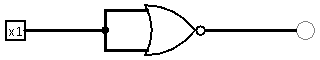
\includegraphics[width=100mm]{sample9.png}
  \label{sample8}\\
  \caption{NORゲートで示したNOT回路}
\end{figure}
\par
\begin{figure}[htbp]
  \centering
  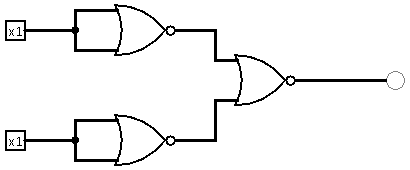
\includegraphics[width=100mm]{sample10.png}
  \label{sample9}\\
  \caption{NORゲートで示したAND回路}
\end{figure}
\par
\begin{figure}[htbp]
  \centering
  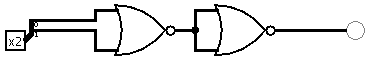
\includegraphics[width=100mm]{sample11.png}
  \label{sample10}\\
  \caption{NORゲートで示したOR回路}
\end{figure}
\par
\begin{figure}[htbp]
  \centering
  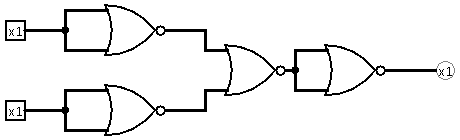
\includegraphics[width=100mm]{sample12.png}
  \label{sampl11}\\
  \caption{NORゲートで示したNOND回路}
\end{figure}
\par
\clearpage
\begin{figure}[htbp]
  \centering
  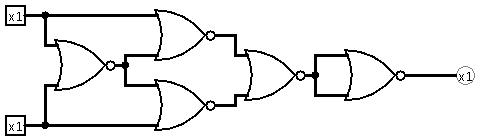
\includegraphics[width=100mm]{sample13.png}
  \label{sample12}\\
  \caption{NORゲートで示したXOR回路}
\end{figure}
\par
\begin{figure}[htbp]
  \centering
  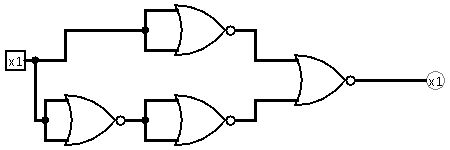
\includegraphics[width=100mm]{sample17.png}
  \label{sample13}\\
  \caption{NORゲートで示した常に0を出力する回路}
\end{figure}
\par
\begin{figure}[htbp]
  \centering
  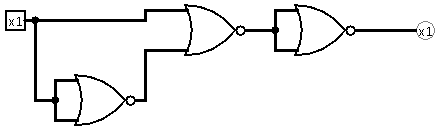
\includegraphics[width=100mm]{sample16.png}
  \label{sample14}\\
  \caption{NORゲートで示した常に1を出力する回路}
\end{figure}
\par


図8は,NORを用いてNOT回路を再現した。これも図1と同様にある入力値の否定を取るため,ある入力値を2つに分けNOR回路に入れる。これにより,NOR回路には同じ値の入力値が入り,そしてその値の否定を取る。\par
この回路に1を入れる。そうすれば,(1,1)が入力され,OR回路の否定を取ることにより,結果として出力は0となる。また,0を入力すると結果は1となる。\par
図9は,NORを用いてAND回路を表現した。ANDを表現するためには,2つの入力値をお互いに否定を取る。それらをさらに,NORに入力されることでAND回路を表現する。
2つの入力値(1,1)を入力したら初めのNORによって、否定され出力結果は0となる。これにより,最後のNORに入力される入力値は(0,0)となり,これらをNORに入力されたら出力結果は0となる。\par
図10は,NORを用いてOR回路をを再現した。OR回路は,NOR回路を否定することでできる。2つの入力をNORに入れ,その出力値を否定することで,OR回路は完成する。\par
この入力値(1,0),(0,1),(1,1)を入力することで始めのNOR回路によって,よって,0の出力になる。そして,その値を否定することで,出力結果は1になる。(0,0)の場合は,NOR回路によって1になり,否定することで0と出力する。\par
図11は,NORをNAND回路に表現している。これは,図9で作成したAND回路を図8で作成した否定回路を繋げることで完成する。\par
入力値(1,1)を入れると,2つ目のNOR回路で1と出力するそれを最後のNORで否定し,0と返す。(0,0),(1,0),(0,1)を入力値にすると,0を返す。\par
図12は,NORで表現したXOR回路になる。これは,AND回路と始めの入力値のNORで出力した値をさらに,NORに入れることで,XOR回路ができる。\par
入力値(1,0),(0,1)を入れるとAND回路では0と出力し,始めの入力値をNORに入れた値は,0を返す。そして,最後のNORに入れることによって,値は1を出力する。次に,入力値を(0,0),(1,1)にすることで,(0,0)では0を(1,1)では1を出力する。そして,始めの入力値をNOR回路に入れて,(0,0)は1を(1,1)は0を出力する。そして,最後のNORで出力結果が0になる。\par
図13は,常に0を出力する回路である。この回路を導くために,論理式で入力値とその否定値の論理積を書くことによって,
この回路は完成する。\par
この回路にある値を入れ,その否定値を出します。始めの入力値と否定値をAND回路に入れることで,この回路は常に0を出力する回路となる。\par
図14は,常に1を出力する回路である。この回路を導くために,論理式で入力値とその否定値の論理和を書くことによってこの回路は完成する。\par
ある値を入力すると,まず始めのNORによって入力値を否定し,その2つの値のOR回路に入れる。これにより,常に出力値を1にすることができる。\par


\section{考察}\par
実験(1)\par
NOT回路について。この回路はすでに1個で作成されているためこれ以上少なくすることはできない。\par
AND回路について。AND回路はNAND回路の否定により,構成することができる。つまり,初めの入力値をNAND回路に入れる。そして,次のNANDを否定の回路にすることで,AND回路が成り立つ。よって,この回路では最低でも2つのNANDが必要だとわかる。\par
OR回路について。NANDは,(1,1)以外の入力を1として返す。このことを前提にして,入力値を(0,0)以外の値を入れある値に変換させれた時に,その値を1として出力するためには,初めに否定を取り,そして最後に2つ入力をNANDとしてうけとる必要がある。そのため,2つの入力を否定するためのNANDと最後に受け取るためのNANDの3つ必要である。\par
NAND回路について。NAND回路は、その一つを置いておけば回路として成立するため1つ十分である。\par
NOR回路について。NOR回路は,OR回路の否定である。つまり,一番最短な回路の構成としてはOR回路にNOT回路を繋げた形である。よって,OR回路の3つとNOT回路の1つの計4つ必要である。\par
XOR回路について。この回路を導くために論理式を用いる。\par
\begin{figure}[htbp]
  \centering
  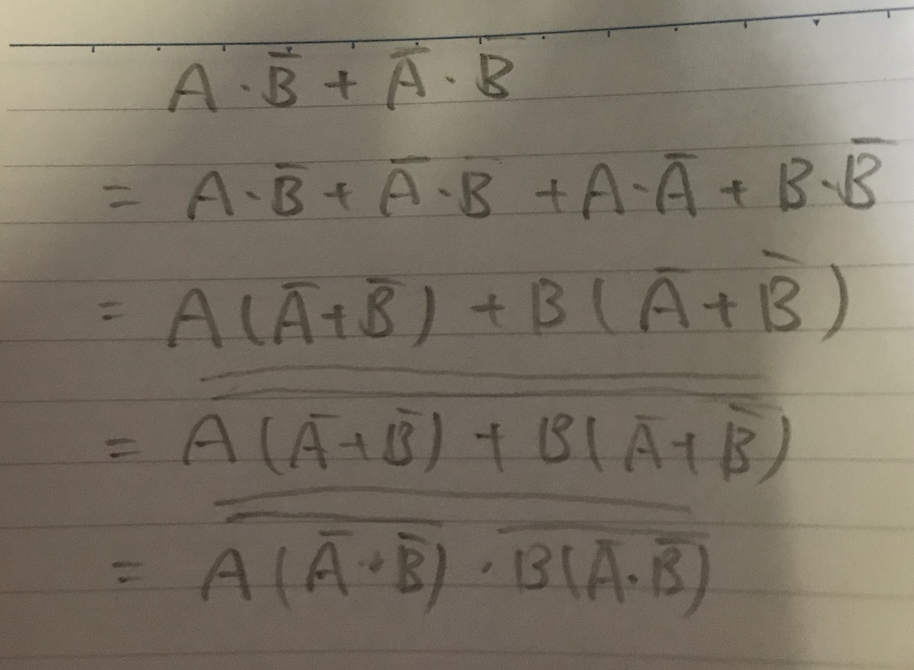
\includegraphics[width=70mm]{sample18.png}
  \label{sample15}\\
  \caption{XORを求めた論理式}
\end{figure}
\par
図15からわかるように,これ以上小さくできないためNANDの数は最低4つは必要である。\par
常に1と0を出力するための回路は,論理式により,これ以上小さくできないため,0の場合は3つ。1の場合は4つ必要である。\par
実験(3)\par
配線を減らすためには,まずは使う量を決めることが大事である。使えるだけ使うでは,手当たり次第使ってしまう恐れがある。仮に,使う量を制限しておけば,その範囲だけでどうやって回路図を作り上げるか考える思考力を上げることができる。配線ミスをなくすためには,頭の中でシミュレーションをすることが大事である。例えば,頭の中で実際の完成図を作り上げそれの通りに配線を繋いでいく。それか,図や絵にして,見てわかるようにすれば配線ミスは減らすことができる。\par
実験(4)\par
NOT回路について。この回路はすでに1個で作成されているためこれ以上少なくすることはできない。\par
AND回路について。NORは(0,0)の時にしか値1を返さないから,まず先のNORを否定にして,その否定した2つの値を次のNORに入れることによって完成する。よって,この回路は,最低3つのNORが必要である。\par
OR回路について。OR回路は,NORの否定であるため,まず始めにNORに値を入れそれを図8で求めた否定を繋げる。これにより,これにより回路は完成する。よって,この回路には最低2つのNORが必要である。\par
NAND回路について。NAND回路はAND回路の否定であるため,図9で作成したAND回路を図8の否定を繋げることで完成する。これにより,最低でも4つは必要である。\par
XOR回路について。この回路を導くために論理式を用いる。\par

\begin{figure}[htbp]
  \centering
  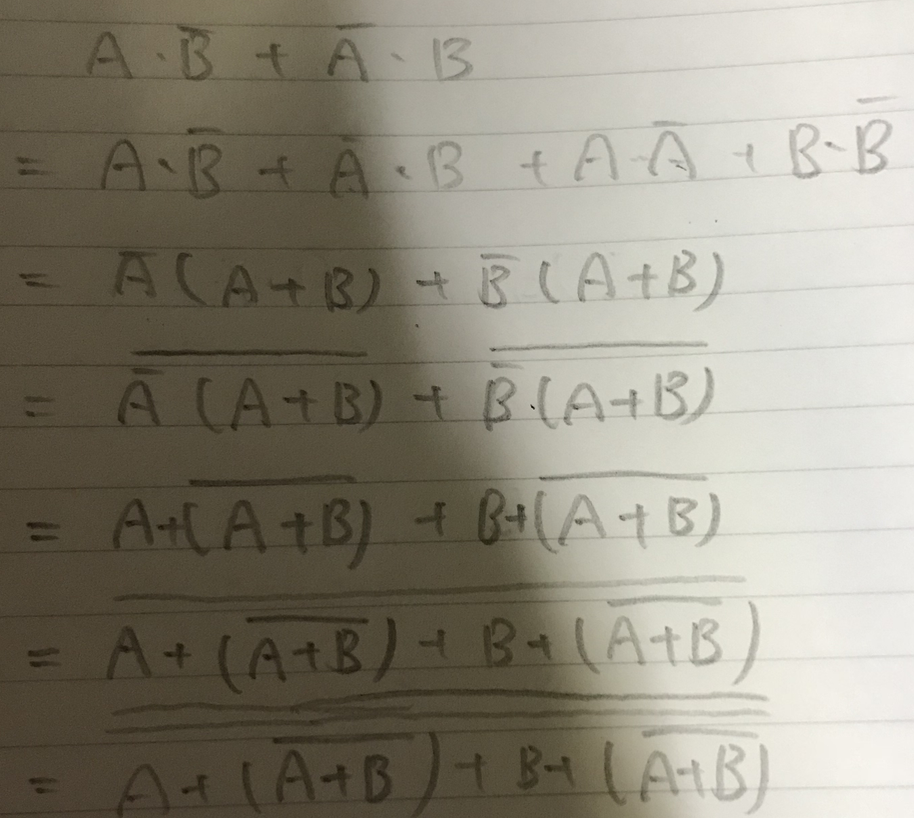
\includegraphics[width=70mm]{sample19.png}
  \label{sample15}\\
  \caption{XORを求めた論理式}
\end{figure}
\par

常に1と0を出力するための回路は,論理式により,これ以上小さくできないため,0の場合は4つ。1の場合は3つ必要である。\par

\section{調査課題}
(a)簡単な論理関数を求める際に必要な技法として,カルノー図を用いる。図17は,カルノー図の例である。カルノー図とは,主加法標準形の論理関数を最小項別に分け,それを最小項の真理値に当てはまるように図に書いていく。真理値表と似ているが,論理変数の順番が違っていたり,使用可能な変数が限られている。6変数以上は事実上扱うことができない。そして,論理関数を簡単にする方法をグループ化という。グループ化の対象となるのは,マスに1と記されたところだけである。$4\times4$や$2\times2$,$1\times4$のようなまとまったグループを作っていく。そして,論理関数に戻りまとまったグループで,関数を簡単化する。これにより,論理関数は短くなり簡単になる。\par
\begin{figure}[htbp]
  \centering
  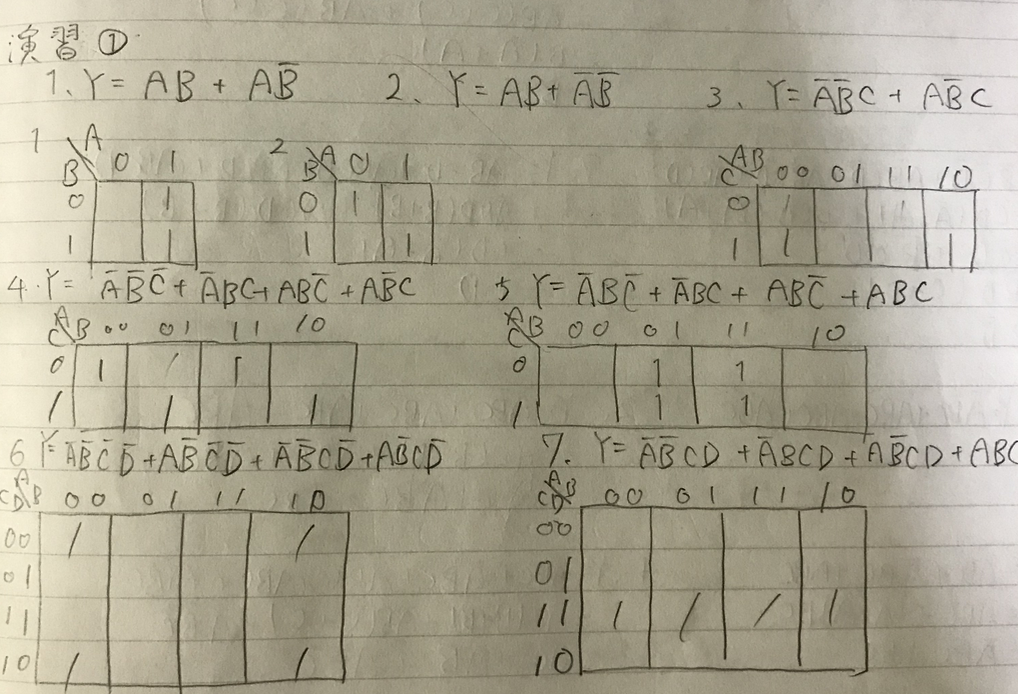
\includegraphics[width=70mm]{sample20.png}
  \label{sample16}\\
  \caption{カルノー図の例}
\end{figure}
\par
(b)半加算器と全加算器。半加算器とは,足し算に使われる回路の一部である。XORとAND回路を用いる。とても,シンプルな回路である。しかし,この回路は,桁の繰り上げを考慮してないために加算器としてはまだ完全とは言えない。全加算器は,前者の半加算器ができなかった桁の繰り上げができる。この加算器は,実は半加算器と半加算器を繋げただけである。初めの半加算器の計算結果で繰り上げになった出力値を次の半加算器に入力することで,加算器として成り立っている。図18は,半加算器と全加算器の回路図,真理値表の例である。\par
\begin{figure}[htbp]
  \centering
  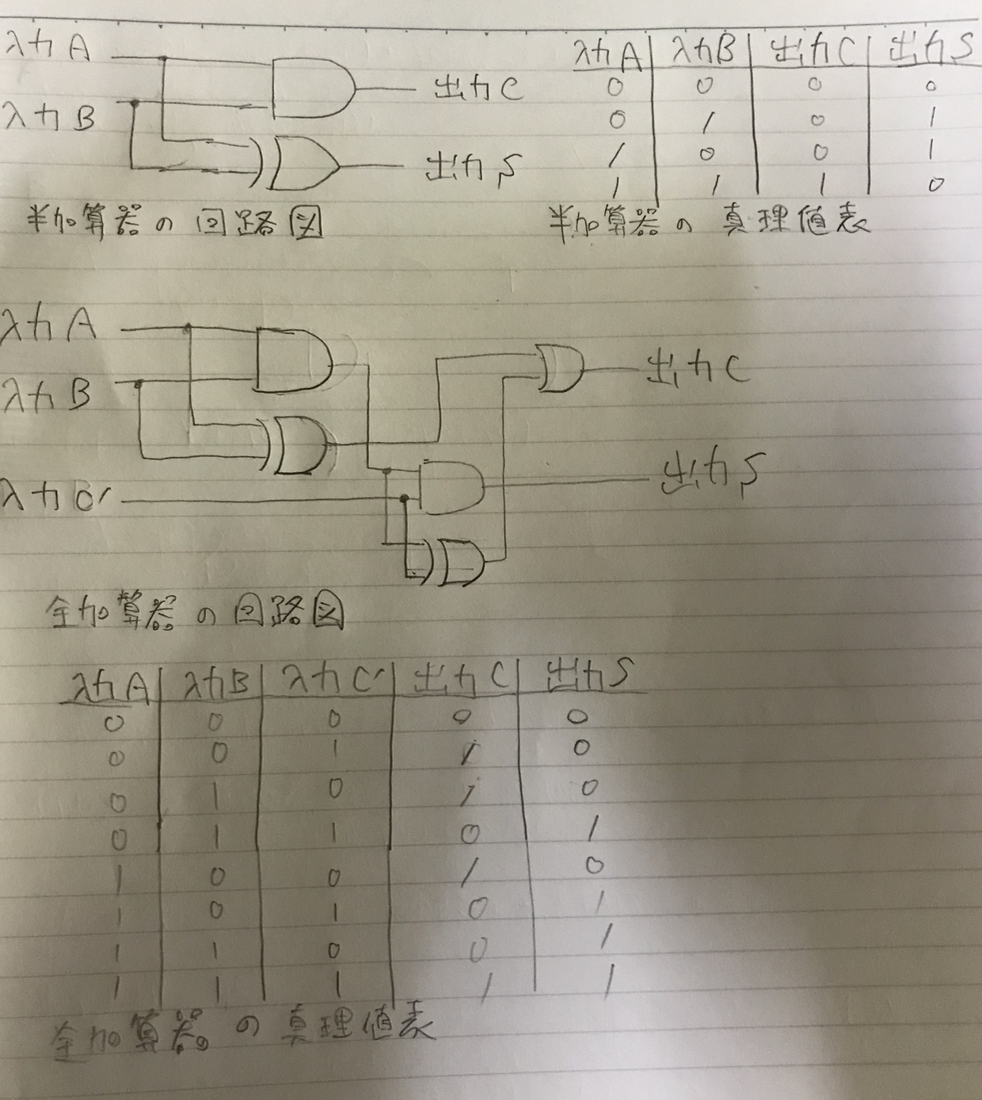
\includegraphics[width=50mm]{sample21.png}
  \label{sample17}\\
  \caption{半加算器と全加算器の回路図,真理値表}
\end{figure}
\par

\section{感想}
 今回の実験を通し,回路の複雑さを理解した。コンピュータには,多くの論理回路が使われており,今回私たちが作成したのはそれのほんの一部に過ぎないことを体感した。それにより,コンピュータ内部の論理回路の仕組みに非常に興味深く感じた。\par
意見としては,教授や院生方々は常に生徒の作業状況を確認しておく必要にあると感じた。理由としては,私の隣に座ってた学生は最初の作業さえままならない状況だと思ったからである。手が止まり,周りを見渡すことしかできていません。そのため,周りの人たちよりも作業状況が悪く見えました。仮に,院生の方々がそれに気づき声かけをすれば,彼の理解も作業状況も上がっていたのだろうと思った。\par

\section{参考文献・引用文献}
\begin{thebibliography}{99}
    \bibitem{Ryukyu}ryukyu: http://www.ie.u-ryukyu.ac.jp/~e035740/jikn/rep6.pdf
    \bibitem{Classroom}classroom: https://classroom.google.com/o/MTE0OTM1MTY3OTla
\end{thebibliography}



\end{document}
